%% abtex2-modelo-relatorio-tecnico.tex, v-1.7.1 laurocesar
%% Copyright 2012-2013 by abnTeX2 group at http://abntex2.googlecode.com/ 
%%
%% This work may be distributed and/or modified under the
%% conditions of the LaTeX Project Public License, either version 1.3
%% of this license or (at your option) any later version.
%% The latest version of this license is in
%%   http://www.latex-project.org/lppl.txt
%% and version 1.3 or later is part of all distributions of LaTeX
%% version 2005/12/01 or later.
%%
%% This work has the LPPL maintenance status `maintained'.
%% 
%% The Current Maintainer of this work is the abnTeX2 team, led
%% by Lauro César Araujo. Further information are available on 
%% http://abntex2.googlecode.com/
%%
%% This work consists of the files abntex2-modelo-relatorio-tecnico.tex,
%% abntex2-modelo-include-comandos and abntex2-modelo-references.bib
%%

% ------------------------------------------------------------------------
% ------------------------------------------------------------------------
% abnTeX2: Modelo de Relatório Técnico/Acadêmico em conformidade com 
% ABNT NBR 10719:2011 Informação e documentação - Relatório técnico e/ou
% científico - Apresentação
% ------------------------------------------------------------------------ 
% ------------------------------------------------------------------------

% Alterado por Rodrigo Campiolo para apresentação de relatórios na disciplina
% de Redes de Computadores II do Bacharelado em Ciência da Computação da UTFPR-CM.


\documentclass[
	% -- opções da classe memoir --
	12pt,				% tamanho da fonte
	%openright,			% capítulos começam em pág ímpar (insere página vazia caso preciso)
	oneside,   	        % para impressão em verso e anverso use twoside. Oposto a oneside
	a4paper,			% tamanho do papel. 
	% -- opções da classe abntex2 --
	%chapter=TITLE,		% títulos de capítulos convertidos em letras maiúsculas
	%section=TITLE,		% títulos de seções convertidos em letras maiúsculas
	%subsection=TITLE,	% títulos de subseções convertidos em letras maiúsculas
	%subsubsection=TITLE,% títulos de subsubseções convertidos em letras maiúsculas
	% -- opções do pacote babel --
	english,			% idioma adicional para hifenização
	french,				% idioma adicional para hifenização
	spanish,			% idioma adicional para hifenização
	brazil,				% o último idioma é o principal do documento
	]{pacotes/abntex2}


% ---
% PACOTES
% ---

% ---
% Pacotes fundamentais 
% ---
\usepackage{cmap}				% Mapear caracteres especiais no PDF
\usepackage{lmodern}			% Usa a fonte Latin Modern
\usepackage[T1]{fontenc}		% Selecao de codigos de fonte.
\usepackage[utf8]{inputenc}		% Codificacao do documento (conversão automática dos acentos)
\usepackage{indentfirst}		% Indenta o primeiro parágrafo de cada seção.
\usepackage{color}				% Controle das cores
\usepackage{graphicx}			% Inclusão de gráficos
% ---

% ---
% Pacotes adicionais, usados no anexo do modelo de folha de identificação
% ---
\usepackage{multicol}
\usepackage{multirow}
% ---
	
% ---
% Pacotes adicionais, usados apenas no âmbito do Modelo Canônico do abnteX2
% ---
\usepackage{lipsum}				% para geração de dummy text
% ---

% ---
% Pacotes de citações
% ---
\usepackage[brazilian,hyperpageref]{backref}	 % Paginas com as citações na bibl
\usepackage[alf]{pacotes/abntex2cite}	% Citações padrão ABNT
\usepackage{comment}
% ---

% ---
% Meus pacotes
% ---
\usepackage{float}
% ---

% --- 
% CONFIGURAÇÕES DE PACOTES
% --- 

% ---
% Configurações do pacote backref
% Usado sem a opção hyperpageref de backref
\renewcommand{\backrefpagesname}{Citado na(s) página(s):~}
% Texto padrão antes do número das páginas
\renewcommand{\backref}{}
% Define os textos da citação
\renewcommand*{\backrefalt}[4]{
	\ifcase #1 %
		Nenhuma citação no texto.%
	\or
		Citado na página #2.%
	\else
		Citado #1 vezes nas páginas #2.%
	\fi}%
% ---

% ---
% Informações de dados para CAPA e FOLHA DE ROSTO
% ---
\titulo{Segurança em Sistemas Operacionais Linux}
\autor{Hendrick Felipe Scheifer\\João Victor Briganti\\Luiz Gustavo Takeda}
\local{Campo Mourão}
\data{Dezembro / 2024}
\instituicao{%
  Universidade Tecnológica Federal do Paraná -- UTFPR
  \par
  Departa           mento Acadêmico de Computação -- DACOM
  \par
  Bacharelado em Ciência da Computação -- BCC
}
\tipotrabalho{Relatório técnico}
% O preambulo deve conter o tipo do trabalho, o objetivo, 
% o nome da instituição e a área de concentração 
\preambulo{Relatório técnico de atividade prática solicitado pelo professor Rodrigo Campiolo na disciplina de Sistemas Operacionais do Bacharelado em Ciência da Computação da Universidade Tecnológica Federal do Paraná.}
% ---

% ---
% Configurações de aparência do PDF final

% alterando o aspecto da cor azul
\definecolor{blue}{RGB}{41,5,195}

% informações do PDF
\makeatletter
\hypersetup{
     	%pagebackref=true,
		pdftitle={\@title}, 
		pdfauthor={\@author},
    	pdfsubject={\imprimirpreambulo},
	    pdfcreator={LaTeX with abnTeX2},
		pdfkeywords={abnt}{latex}{abntex}{abntex2}{relatório técnico}, 
		colorlinks=true,       		% false: boxed links; true: colored links
    	linkcolor=blue,          	% color of internal links
    	citecolor=blue,        		% color of links to bibliography
    	filecolor=magenta,      		% color of file links
		urlcolor=blue,
		bookmarksdepth=4
}
\makeatother
% --- 

% --- 
% Espaçamentos entre linhas e parágrafos 
% --- 

% O tamanho do parágrafo é dado por:
\setlength{\parindent}{1.3cm}

% Controle do espaçamento entre um parágrafo e outro:
\setlength{\parskip}{0.2cm}  % tente também \onelineskip

% ---
% compila o indice
% ---
\makeindex
% ---

% Omite a numeração de capítulos
\renewcommand*\thesection{\arabic{section}}



% ----
% Início do documento
% ----
\begin{document}

% Retira espaço extra obsoleto entre as frases.
\frenchspacing 

% ----------------------------------------------------------
% ELEMENTOS PRÉ-TEXTUAIS
% ----------------------------------------------------------
% \pretextual

% ---
% Capa
% ---
%\imprimircapa
% ---

% ---
% Folha de rosto
% (o * indica que haverá a ficha bibliográfica)
% ---
\imprimirfolhaderosto
% ---


% ---
% RESUMO
% ---

% resumo na língua vernácula (obrigatório)
\begin{resumo}
Os objetivos deste trabalho são compreender e aplicar conceitos e recursos de segurança em sistemas operacionais Linux. Para tal atividade foi utilizado um sistema operacional Linux executado em uma máquina virtual através do hipoervisor VirtualBox, neste sistema o procedimento realizado foi a configuração de recursos importantes para a segurança no sistema operacional, além de observação de arquivos importantes para o gerenciamento dos recursos de segurança. Este trabalho atingiu seu objetivo com sucesso, permitindo a compreensão clara e aplicação de recursos básicos de segurança em sistemas operacionais Linux, sem apresentar grandes dificuldades. Os resultados provam a importância da aplicação de recursos para prover segurança as informações e recursos do sistema operacional, consolidando o conhecimento teórico.

 \vspace{\onelineskip}
    
 \noindent
 \textbf{Palavras-chave}: segurança; sistemas operacionais; linux.
\end{resumo}
% ---

% ---
% inserir lista de ilustrações
% ---
%\pdfbookmark[0]{\listfigurename}{lof}
%\listoffigures*
%\cleardoublepage
% ---

% ---
% inserir lista de tabelas
% ---
%\pdfbookmark[0]{\listtablename}{lot}
%\listoftables*
%\cleardoublepage
% ---

% ---
% inserir lista de abreviaturas e siglas
% ---
%\begin{siglas}
%  \item[IP] Internet Protocol
%  \item[TCP] Transmission Control Protocol
%  \item[UDP] User Datagram Protocol
%\end{siglas}
% ---

% ---
% inserir o sumario
% ---
\pdfbookmark[0]{\contentsname}{toc}
\tableofcontents*
\cleardoublepage
% ---

% ----------------------------------------------------------
% ELEMENTOS TEXTUAIS
% ----------------------------------------------------------
\textual

\makeatletter
\renewcommand{\chapter}{\@gobbletwo}
\makeatother

\section{Introdução}
\label{sec:introducao}

A segurança é um aspecto indispensável em um sistema operacional, o qual diz respeito a proteção dos recursos do computador contra ameaças externas, como acesso não autorizado, destruição ou aletração maliciosa e introdução acidental de inconsistências. Os recursos citados anteriormente como foco da segurança se referem às informações armazenadas, processador, memória, discos e redes, os quais constituem o computador~\cite{silberschatz2015}.

O estudo e aplicação da segurança em sistemas operacionais resulta em melhor consistência no funcionamento, assim como garante a devida privacidade ao usuário. Este trabalho tem como foco aspectos de segurança em sistemas operacionais Linux, as próximas seções falarão sobre os objetivos da atividade, fundamentação essencial para a compreensão, procedimentos realizados e resultados obtidos.

\section{Objetivos}
\label{sec:objetivos}

Os objetivos deste trabalho são a compreensão de princípios básicos da segurança em sistemas operacionais, identificar arquivos relevantes para a configuração da segurança em sistemas operacionais Linux e aprender comandos básicos utilizados em configurações de segurança em sistemas operacionais Linux.

\section{Fundamentação}
\label{sec:fundamentacao}

Sistemas operacionais são inicialmente projetados visando a segurança interna, ou seja, os recursos são utilizados e acessados como esperado em qualquer circunstância. Mas estas circunstâncias observadas anteriormente não incluem atividades mal-intencionadas, as quais são atribuídas o nome ''ataques", que podem violar a segurança do sistema~\cite{silberschatz2015}.

A segurança da informação possui três princípios fundamentais, sendo eles a confidencialidade, o qual determina que os recursos do sistema podem apenas ser utilizados por devidamente autorizados, a integridade, que determina que os recursos do sistema podem apenas ser alterados ou destruídos por usuários autorizados, e por fim a disponibilidade, que determina que os recursos devem estar sempre disponíveis para usuários autorizados que desejam utilizá-los~\cite{maziero2019}.

Qualquer possibilidade de violação da segurança do sistema é considerada uma ameaça, como a existência de vulnerabilidades, enquanto qualquer tentativa de violar a segurança do sistema é considerada um ataque utilizando por exemplos as vulnerabilidades existentes. Os ataques possuem diferentes objetivos e violam de diferentes formas a segurança do sistema, estas violações podem ser de diferentes tipos~\cite{silberschatz2015}:

\begin{itemize}
    \item \textbf{Brecha de sigilo}: violação de segurança que visa acesso não autorizado de dados, este ataque está geralmente associado a um invasor, que ao obter dados do usuário pode se beneficiar de alguma forma.
    \item \textbf{Brecha de integridade}: violação que visa alterar dados sem autorização para tal ação, ataque que também visa beneficiar algum invasor ou prejudicar outro usuário.
    \item \textbf{Brecha de disponibilidade}: violação que visa a destruição não autorizada de dados, este ataque visa explorar benefícios prejudicando o usuário proprietário dos dados.
    \item \textbf{Roubo de serviço}: violação que se baseia no uso não autorizado de recursos, ataque que visa se beneficiar a partir dos recursos alheios, o que pode ser feito, por exemplo, a partir da instalação de um \textit{daemon} no sistema para fins de uso de recursos como disco ou processador sem a autorização do proprietário do sistema.
    \item \textbf{Recusa de serviço}: violação que explora o impedimento do uso correto do sistema, visando prejudicar o proprietário do sistema ou terceiros que necessitem destes serviços, ataques deste tipo são chamados de DOS (\textit{denial-of-service}, e podem surgir acidentalmente em alguns casos, a partir de \textit{bugs} no sistema, mas podem ser associados a invasores que criam \textit{daemons} para isto.
\end{itemize}

Conforme as vulnerabilidades que trazem ameaças ao sistema se tornaram conhecidas, soluções foram desenvolvidas e aplicadas em sistemas operacionais, a seção \ref{sec:procedimentos} apresenta a discussão de alguns recursos básicos de segurança implementados para sistemas operacionais Linux e demonstra o uso destes recursos em uma máquina virtual.

\section{Materiais}
\label{sec:materiais}

\begin{itemize}
  \item Especificações do computador utilizado:
  \begin{itemize}
    \item Modelo: Notebook Dell G15
    \item CPU: Intel Core i$5$-$12500$H
    \item Memória Principal: $16$GB RAM
    \item Memória Secundária: SSD $1$TB NVME
    \item Sistema Operacional: Windows $10$
  \end{itemize}
  \item Hipervisor: VirtualBox $7.1.2$
  \item Sistema Operacional utilizado no Hipervisor: GNU/Linux Debian $12.7$
  \item Núcleo: Linux $4.9.0$ 
\end{itemize}

\section{Procedimentos e Resultados}
\label{sec:procedimentos}

Nesta seção, serão abordados diversos conceitos e recursos básicos de segurança aplicados em um sistema operacional Linux em ambiente virtual, utilizando o hipervisor VirtualBox. Serão abordados e detalhados arquivos e comandos essenciais para prover segurança a sistemas operacionais Linux. Após a instalação da distribuição Linux fornecida pelo professor, o usuário ''\textit{root}`` foi utilizado para a realização das configurações, pois possui privilégios adminstrativos.

\subsection{Configuração do nível de segurança das senhas}
\label{subsec:senhas}

Senhas são um recurso de segurança extremamente comum e utilizado, devido a sua facilidade de compreensão e utilização, porém, ainda há a possibilidade de um invasor obter de alguma forma a senha, seja através da engenharia social, onde o invasor conhece o alvo e através da obtenção de informações sobre ele consegue adivinhar a senha, ou até mesmo por métodos de força bruta, no qual milhares de possíveis combinações são testadas até que se obtenha a combinação correta que forma a senha~\cite{silberschatz2015}.

Uma solução comumente utilizada para dificultar o ataque e reduzir os riscos de invasão é a utilização de padrões mais complexos de senha, que envolve a exigência de caracteres de diferentes classes para a criação da senha, além de um número mínimo de caracteres. Para a implementação deste recurso em sistemas operacionais Linux, pode-se utilizar como ferramenta a biblioteca \textit{libpam-quality}, que proporciona recursos de segurança, incluindo a verificação de senhas de acordo com a solução apresentada anteriormente, com a instalação desta biblioteca, com o comando \textit{apt install libpam-quality}, um arquivo de configuração da qualidade de senhas será criado em \textit{/etc/security/pwquality.conf} ~\cite{libpam-pwquality}.

O arquivo citado anteriormente contém as configuração da qualidade de senha, como a quantidade mínima de caracteres total, de dígitos numéricos, caracteres especiais e de letras minúsculas e maiúsculas. O exemplo de configuração proposto pela atividade diz que a senha deve conter as seguintes exigências:

\begin{itemize}
    \item Mínimo de 10 caracteres ao todo;
    \item Mínimo de 2 dígitos numéricos;
    \item Mínimo de 1 letra maiúscula;
    \item Mínimo de 1 letra minúscula;
    \item Mínimo de 1 caractere especial.
\end{itemize}

Para a adicionar os requisitos basta modificar o arquivo \textit{/etc/security/pwquality.conf}, para realizar alterações como essa durante a prática, foi utilizado o editor de texto \textit{Nano}, a partir do comando \textit{nano /etc/security/pwquality.conf}. O arquivo possui algumas variáveis que controlam os requisitos de senhas, para a implementação proposta anteriormente foram alteradas as seguintes variáveis:

\begin{itemize}
    \item \textit{minlen} = 10: para especificar que toda senha deve possuir no mínimo 10 caracteres ao todo;
    \item \textit{dcredit} = -2: exige que a sejam escrito ao menos dois dígitos numéricos na senha;
    \item \textit{ucredit} = -1: exige que seja escrito ao menos uma letra maiúscula na senha;
    \item \textit{lcredit} = -1: exige que seja escrito ao menos uma letra minúscula na senha;
    \item \textit{ocredit} = -1: exige que seja escrito ao menos um caractere especial na senha;
    \item \textit{minclass} = 4: determina que o número de classes diferentes que compõe a senha é 4 (dígitos, maiúsculas, minúsculas e caracteres especiais).
\end{itemize}

A figura \ref{fig:pwquality} mostra as alterações realizadas no arquivo \textit{/etc/security/pwquality.conf}, citadas anteriormente.

\begin{figure}[H]
  \centering
  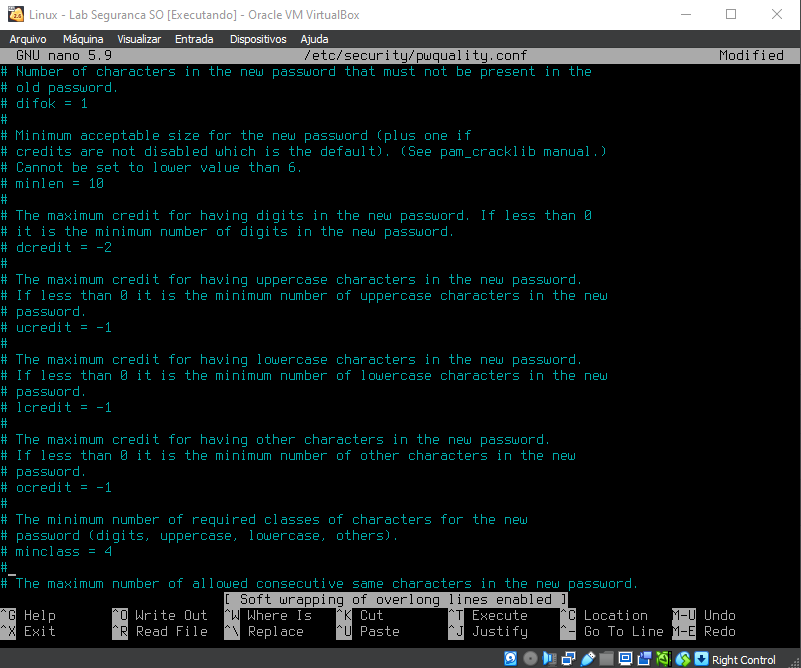
\includegraphics[scale=0.7]{figuras/nano_pwquality.png}
  \caption{Arquivo \textit{/etc/security/pwquality.conf}.}
  \label{fig:pwquality}
\end{figure}

Após salvar as alterações, a criação de senhas só será bem sucedida caso a senha digitada possua os requisitos mínimos.

\subsection{Criação de grupos e usuários}
\label{subsec:grupos_usuarios}

A próxima etapa envolve a criação de grupos e usuários para o sistema. Grupos são comumente criados em sistemas para que usuários com diferentes privilégios ou funções no sistema possam ser gerenciados de forma conjunta. A seguir serão descritos alguns passos essenciais para que esta criação aconteça de forma correta e que não comprometa a segurança do sistema

\subsubsection{Configuração \textit{GROUPHOMES}}
O parâmetro \textit{GROUPHOMES} encontrado no arquivo de configuração \textit{/etc/adduser.conf}, é utilizado para definir o comportamento padrão na criação de diretórios ''\textit{home}`` de novos usuários em sistemas operacionais Linux ao utilizar o comando \textit{adduser}. Quando este parâmetro está ativado, os diretórios pessoais dos usuários serão organizados em subdiretórios de um diretório geral do grupo, por exemplo, o usuário ''Aluno`` do grupo ''alunos`` terá seu diretório pessoal em \textit{/home/alunos/Aluno/} ao invés de apenas \textit{/home/Aluno/}. Esta configuração auxilia na segurança de modo geral, pois permite um maior controle e proteção dos dados armazenados em um sistema multiusuário.

A figura \ref{fig:adduser} demonstra a alteração realizada no arquivo de configuração citado anteriormente, esta alteração foi realizada através do editor de texto \textit{Nano}. Para a ativação do parâmetro, basta alterar o valor associado à variável \textit{GROUPHOME} para \textit{yes}

\begin{figure}[H]
  \centering
  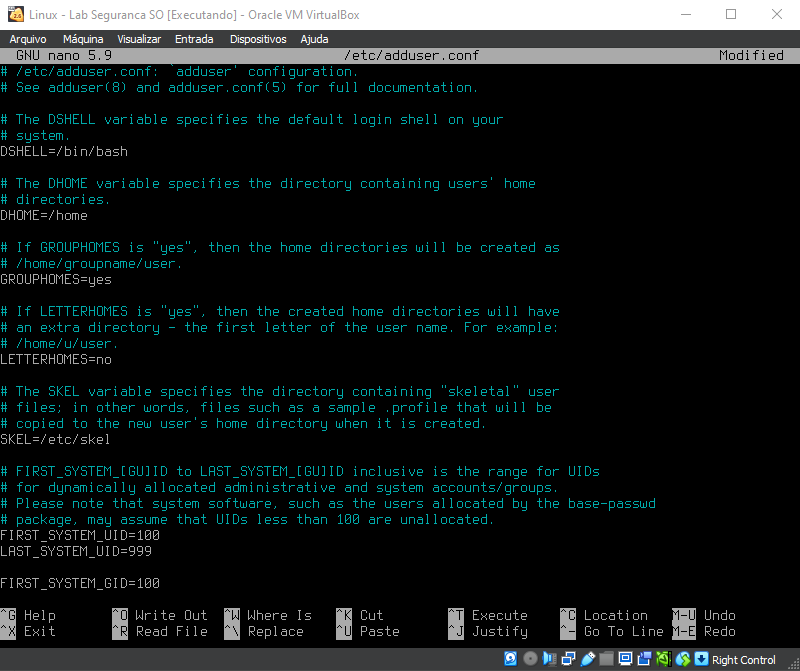
\includegraphics[scale=0.7]{figuras/nano_adduser.png}
  \caption{Arquivo \textit{/etc/adduser.conf}.}
  \label{fig:adduser}
\end{figure}

\subsubsection{Criação de grupos}
Como exemplo para a utilização do sistema, a pratica propõe a criação de dois grupos: ''alunos`` e ''professores". Para criar os grupos, o comando \textit{addgroup} foi utilizado, sua utilização é simples, basta adicionar o nome desejado para o grupo após o comando, por exemplo, \textit{addgroup alunos}, conforme apresentado na figura \ref{fig:addgroup}. O retorno \textit{Done} após a execução do comando indica que o grupo foi criado com sucesso.

\begin{figure}[H]
  \centering
  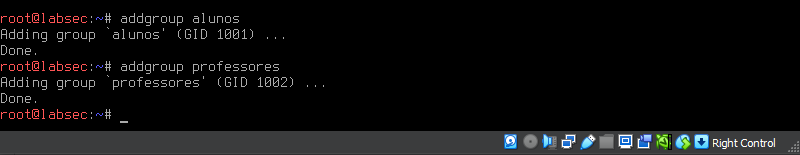
\includegraphics[scale=0.7]{figuras/addgroups.png}
  \caption{Comando \textit{addgroup}.}
  \label{fig:addgroup}
\end{figure}

\subsubsection{Cadastro de usuários}
A atividade propõe o cadastro de um usuário para cada grupo, esta etapa pode ser dividida em dois passos: cadastrar os usuários e adicioná-los aos seus grupos. Para o cadastro do usuário foi utilizado o comando \textit{adduser}, sua utilização também é simples, pois basta adicionar o nome do usuário após o comando, por exemplo, \textit{adduser usuário}, a figura \ref{fig:add_aluno} demonstra o uso do comando com o cadastro do usuário ''aluno`` no sistema.

\begin{figure}[H]
  \centering
  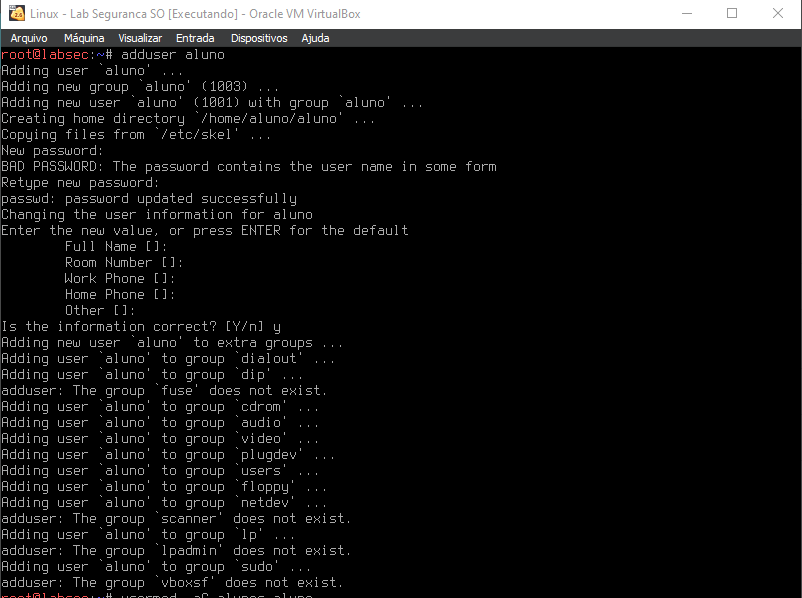
\includegraphics[scale=0.8]{figuras/adduser_aluno.png}
  \caption{Comando \textit{adduser aluno}.}
  \label{fig:add_aluno}
\end{figure}

De forma semelhante ao cadastro anterior, a figura \ref{fig:add_prof} apresenta o cadastro do usuário ''professor".

\begin{figure}[H]
  \centering
  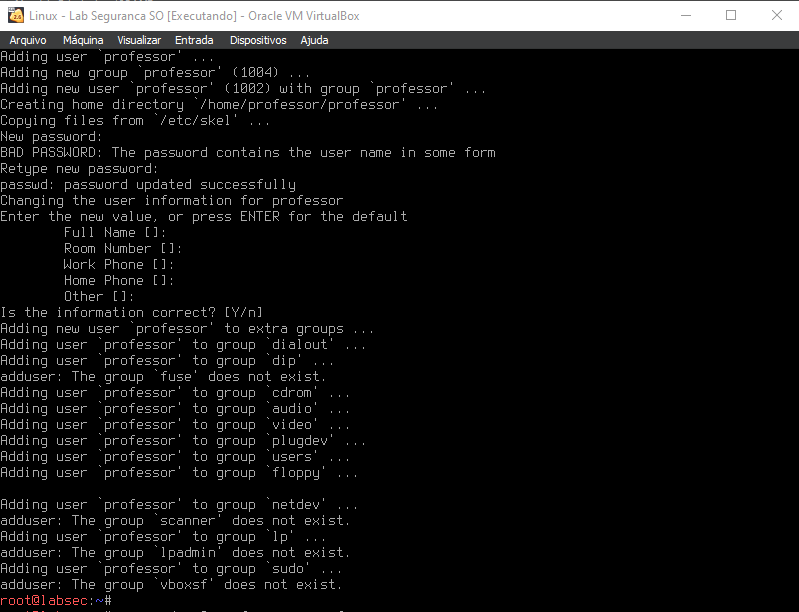
\includegraphics[scale=0.8]{figuras/adduser_prof.png}
  \caption{Comando \textit{adduser professor}.}
  \label{fig:add_prof}
\end{figure}

Após o cadastro dos usuários, devemos associá-los a seus devidos grupos, para isso foi utilizado o comando para modificação de usuários \textit{usermod} com a opção ''-aG`` que significa ''\textit{append group} (acrescentar grupo)`` seguido do grupo que desejamos acrescentar e o usuário em questão. A figura \ref{fig:usermod} demonstra o uso deste comando para adicionar os usuários ''aluno`` ao grupo ''alunos`` e ''professor`` ao grupo ''professores". 

\begin{figure}[H]
  \centering
  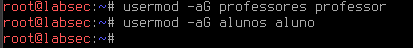
\includegraphics[scale=0.8]{figuras/usermod.png}
  \caption{Comando \textit{usermod -aG}.}
  \label{fig:usermod}
\end{figure}

\subsubsection{Remoção dos usuários do grupo \textit{alunos} do grupo \textit{sudo}}
É de grande importância que apenas usuários devidamente autorizados tenham acesso a funções administrativas, as quais são proporcionadas para usuários pertencentes ao grupo ''\textit{sudo}``, portanto, por motivos de segurança, a atividade propõe que os usuários do grupo aluno sejam removidos do grupo \textit{sudo}. Para isso, inicialmente identificamos os usuários pertencentes ao grupo alunos, utilizando o comando \textit{getent group alunos}, que serve para consultar dados de um grupo específico, no caso, \textit{alunos}. Após isso, removemos os usuários identificados no passo anterior com o comando \textit{gpasswd}, utilizada para gerenciar usuários e senhas de grupos, com a opção ''-d`` para remover um usuário no caso \textit{aluno} do grupo \textit{sudo}, resultando no seguinte comando \textit{gpasswd -d aluno sudo}. Esta etapa é apresentada na figura \ref{fig:gpasswd}.

\begin{figure}[H]
  \centering
  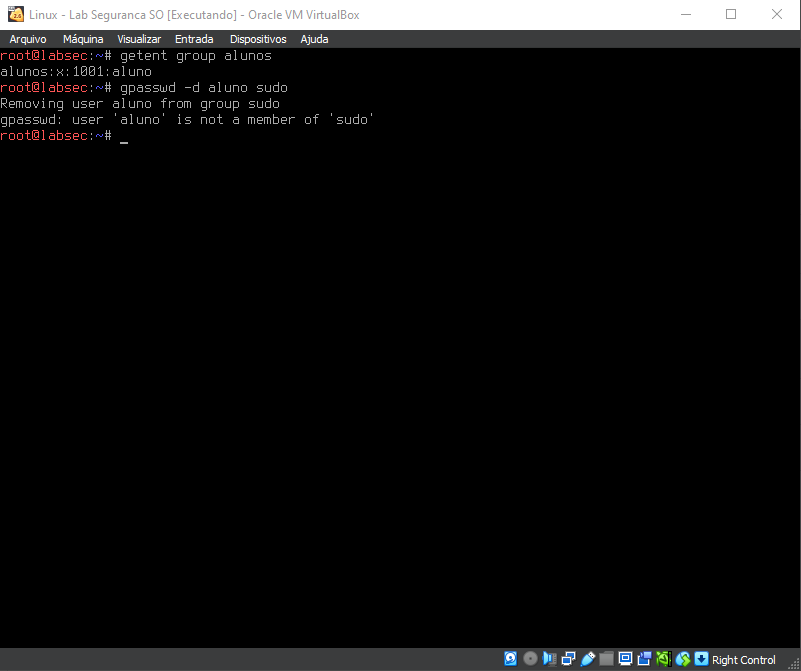
\includegraphics[scale=0.7]{figuras/gpasswd.png}
  \caption{Comando \textit{gpasswd}.}
  \label{fig:gpasswd}
\end{figure}

\subsection{Configuração de permissões para arquivos}
Para manter os princípios da segurança de sistemas, abordados na seção \ref{sec:fundamentacao}, devemos garantir que um arquivo seja acessado de forma devidamente autorizada. Permissões de arquivos servem para determinar o que cada usuário ou grupo pode ou não acessar no sistema, existem três permissões diferentes para arquivos em um sistema operacional:
\begin{itemize}
    \item \textbf{Leitura}: permissão para acessar o arquivo;
    \item \textbf{Escrita}: permissão para alterar um arquivo;
    \item \textbf{Execução}: permissão para executar um arquivo.
\end{itemize}

Essas três permissões são atribuídas a três níveis de autorização em relação ao arquivo: dono, grupo ao qual o dono pertence e outros, que se refere aos demais usuários. Nesta subseção será abordado a manipulação destas permissões.

\subsubsection{Criação de arquivo e alteração de permissões}
Para este procedimento, é necessário um arquivo, o qual terá suas permissões manipuladas, este arquivo será chamado ''\textit{meuarquivo.txt}``, e será criado pelo usuário ''\textit{aluno}``. Portanto, para a criação do arquivo foi inicialmente iniciado uma nova sessão, com o usuário correto, e em seguida o comando \textit{touch} foi utilizado para criar o arquivo, conforme a figura \ref{fig:touch} apresenta.
\begin{figure}[H]
  \centering
  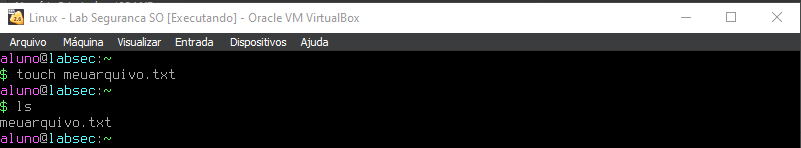
\includegraphics[scale=0.7]{figuras/touch.png}
  \caption{Comando \textit{touch}.}
  \label{fig:touch}
\end{figure}

Para manipular permissões é utilizado o comando \textit{chmod}, que deve ser acompanhado de dois dados: as permissões e o arquivo ou diretório em questão. As permissões podem ser escritas de duas formas:
\begin{itemize}
    \item \textbf{Numérica}: as permissões dos três níveis são especificadas em três valores que vão de 0 a 7 e representam a soma das permissões desejadas, cada permissão possui um valor, execução vale 1, escrita vale 2, e leitura vale 4. Esta forma é apresentada na figura \ref{fig:chmod_num}.
    \item \textbf{Com opções}: outra forma é especificar as permissões de cada nível que se deseja alterar de atribuindo os símbolos desejados, os níveis são \textit{u} para o dono do arquivo, \textit{g} para o grupo do arquivo e \textit{o} para outros. Os símbolos equivalentes as permissões são \textit{r} para leitura, \textit{w} para escrita e \textit{x} para execução. Esta forma é apresentada na figura \ref{fig:chmod_ugoa}.
\end{itemize}

Para verificar as permissões dos arquivos foi utilizado o comando \textit{ls} de listagem com a opção ''-l``, que apresenta informações detalhadas dos arquivos e diretórios, incluindo as permissões. A saída do comando apresenta as permissões da seguinte forma: do segundo ao décimo caractere da linha são agrupados em 3 trios que representam as permissões para os níveis de dono, grupo e outros, respectivamente, dentro do trio de caracteres são representadas as permissões de leitura, escrita e execução, respectivamente, caso haja um traço no lugar da permissão, esta permissão não foi concedida a este nível. Este comando pode ser observados nas figuras \ref{fig:chmod_num} e \ref{fig:chmod_ugoa}.

A atividade propõe que as permissões do arquivo criado sejam: leitura e escrita para o dono, leitura para o grupo e nenhuma permissão para outros. Esta configuração foi realizada pelas duas formas de escritas que o comando \textit{chmod} permite, a forma numérica pode ser observada na figura \ref{fig:chmod_num} e a forma por opções na figura \ref{fig:chmod_ugoa}.

\begin{figure}[H]
  \centering
  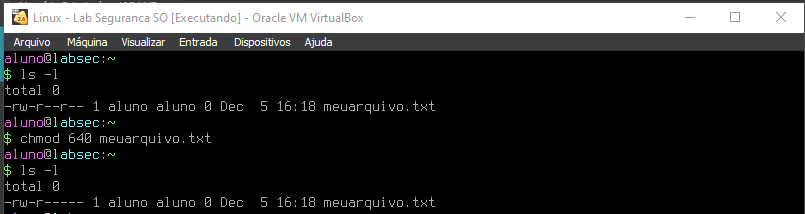
\includegraphics[scale=0.7]{figuras/chmod_num.png}
  \caption{Comando \textit{chmod} no formato numérico.}
  \label{fig:chmod_num}
\end{figure}

\begin{figure}[H]
  \centering
  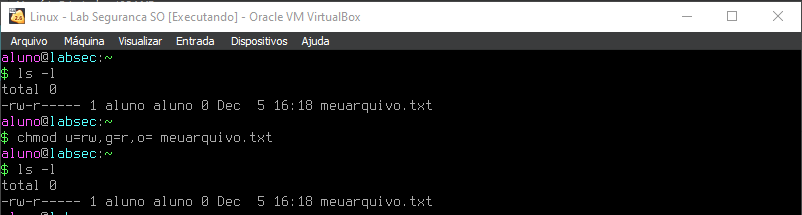
\includegraphics[scale=0.7]{figuras/chmod_ugoa.png}
  \caption{Comando \textit{chmod} com opções.}
  \label{fig:chmod_ugoa}
\end{figure}

\subsubsection{Alteração de dono e grupo do arquivo}
Em muitas situações a posse de um arquivo pode ser alterada, e para manter a segurança do sistema, deve-se alterar o dono e, caso necessário, o grupo do arquivo. Para tal operação pode-se utilizar o comando \textit{chown}, que deve receber como dados o nome do novo usuário ou grupo e o nome do arquivo ou diretório, para especificar se a alteração é de dono ou usuário é simples, para alterar o dono, basta adicionar o nome do usuário que irá receber a posse do arquivo, para grupo há a necessidade de adicionar '':`` antes do nome do grupo que assumirá a posse, por exemplo, '':professores``. O uso deste comando pode ser observado na figura \ref{fig:chown}.

Para a verificação do dono e grupo do arquivo foi utilizado o mesmo comando \textit{ls -l} apresentado na etapa anterior. A atividade propõe que o arquivo tenha sua posse transferida para o usuário ''professor`` e o grupo ''professores``. A execução desta etapa é apresentada na figura \ref{fig:chown}.
\begin{figure}[H]
  \centering
  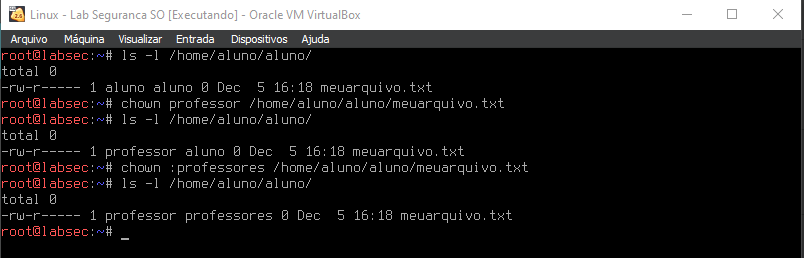
\includegraphics[scale=0.7]{figuras/chown.png}
  \caption{Comando \textit{chown}.}
  \label{fig:chown}
\end{figure}

\subsection{Gerenciamento de autenticação}
A autenticação de usuários é a principal forma de acesso ao sistema, devendo ocorrer de forma devidamente autorizada, portanto há a necessidade de gerenciar a autenticação do sistema. Nesta subseção será abordado a observação de autenticações recentes, configuração da obrigatoriedade de autenticação e arquivos importantes referente à autenticação.

\subsubsection{Observação de autenticações}
Para observar os usuários que se autenticaram no sistema recentemente podemos utilizar o comando \textit{lastlog}, que apresenta a lista de usuários do sistema e em caso de autenticação apresenta a data e a porta na qual aconteceu sua última autenticação, conforme pode ser visto na figura \ref{fig:lastlogs}.

\begin{figure}[H]
  \centering
  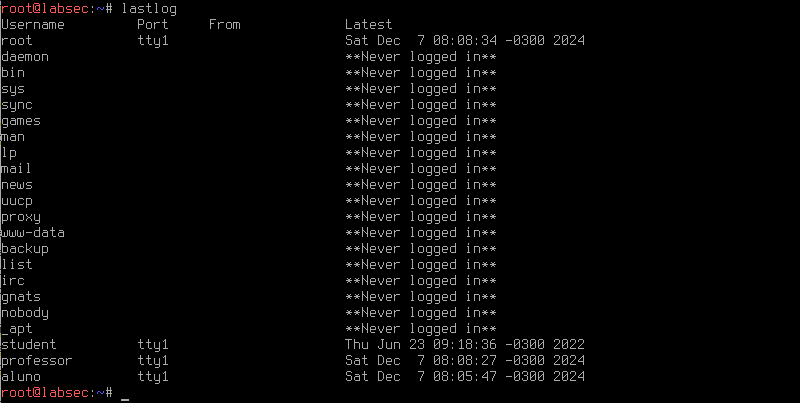
\includegraphics[scale=0.7]{figuras/lastlog.png}
  \caption{Comando \textit{lastlog}.}
  \label{fig:lastlogs}
\end{figure}

\subsubsection{Obrigatoriedade de autenticação}
\label{subsubsec:passwd_root}
É possível em sistemas operacionais permitir que usuário não seja obrigado a autenticar-se para realizar o \textit{login}, claro que não é recomendado por motivos de segurança, mas em alguns casos pode ser necessário.

Em sistemas Linux essa configuração pode ser realizada da seguinte forma: no arquivo \textit{/etc/passwd} encontre o usuário desejado, o segundo item da linha do usuário é um ''x``, que indica que a senha do usuário está criptografada e armazenada no arquivo \textit{/etc/passwd}, remova este ''x`` e o usuário não irá possuir uma senha vinculada, logo, não há a obrigatoriedade de autenticação.

Para exemplo deste recurso, foi alterar o arquivo para o usuário \textit{root} não precise mais se autenticar. Esta alteração pode ser observada na figura \ref{fig:passwd_root}, na primeira linha.
\begin{figure}[H]
  \centering
  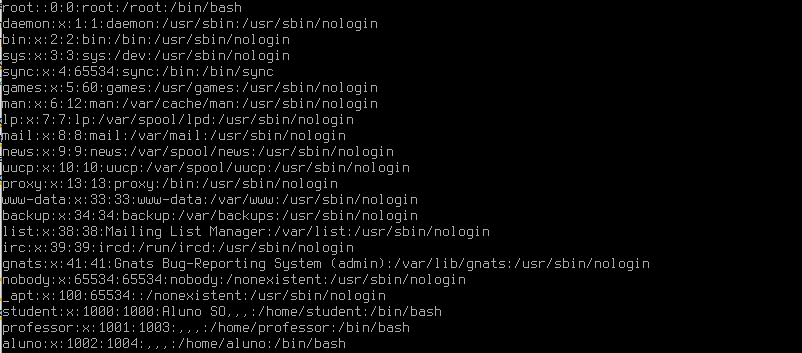
\includegraphics[scale=0.7]{figuras/passwd_root.png}
  \caption{Alteração no arquivo \textit{/etc/passwd}.}
  \label{fig:passwd_root}
\end{figure}

Como resultado desta alteração, o usuário \textit{root} não precisa mais digitar sua senha para realizar o \textit{login}, observe o teste na figura \ref{fig:login_sem_senha}.

\begin{figure}[H]
  \centering
  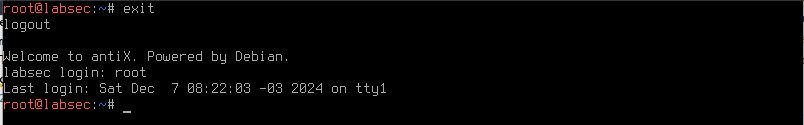
\includegraphics[scale=0.7]{figuras/login_sem_senha.png}
  \caption{Usuário \textit{root} acessando o sistema sem senha.}
  \label{fig:login_sem_senha}
\end{figure}

Por razões de segurança, a autenticação do usuário \textit{root} foi ativada novamente desfazendo o passo anterior.

\subsubsection{Arquivo \textit{/etc/shadow}}
O arquivo \textit{/etc/shadow} armazena dados importantes relacionados às senhas dos usuários do sistema, os quais podem ser alterados conforme a necessidade para razões de segurança, uma representação textual do arquivo pode ser observada na figura \ref{fig:shadow}. 

\begin{figure}[H]
  \centering
  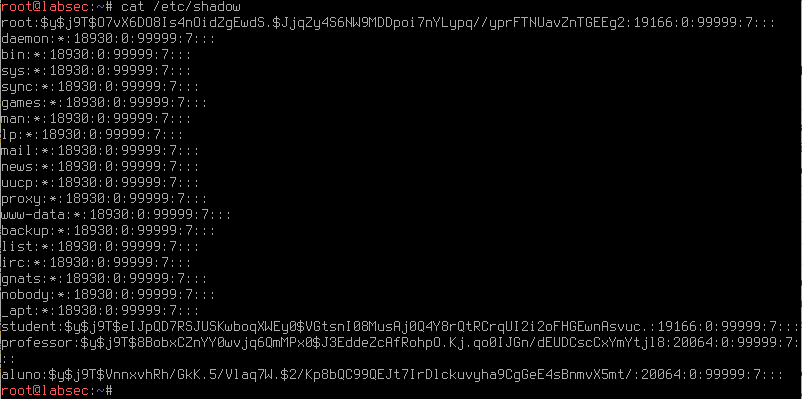
\includegraphics[scale=0.7]{figuras/shadow.png}
  \caption{Arquivo \textit{/etc/shadow}.}
  \label{fig:shadow}
\end{figure}

Para apresentar os campos de dados presentes no arquivo, utilizaremos como exemplo o usuário \textit{student}, os dados presentes no arquivo são:
\begin{itemize}
    \item \textbf{Nome do usuário}: primeiro campo de cada linha, identifica o usuário em questão pelo seu nome de usuário no sistema;
    \item \textbf{Senha}: a senha é armazenada no segundo campo de forma criptografada, visando manter a senha segura mesmo que um invasor obtenha acesso ao arquivo \textit{/etc/shadow};
    \item \textbf{Última modificação}: o terceiro campo apresenta a data da última modificação realizada na senha deste usuário, a data é dada em um formato específico, sendo a quantidade de dias decorridos após 01/01/1970, data selecionada para servir de referência para sistemas UNIX;
    \item \textbf{Tempo mínimo para alteração}: o quarto campo representa a quantidade mínima de dias que o usuário deve esperar para poder alterar sua senha;
    \item \textbf{Tempo máximo para alteração}: o quinto campo representa a quantidade máxima de dias que o usuário pode manter a mesma senha, antes de ser obrigado a alterá-la;
    \item \textbf{Tempo para aviso prévio}: o sistema operacional pode alertar o usuário sobre a obrigatoriedade da troca de senha, o sexto campo representa com quantos dias antes da data limite o sistema emitirá este aviso;
    \item \textbf{Tempo de inatividade para desativação}: o sétimo campo, não adicionado ao usuário \textit{student}, representaria a quantidade de dias que o usuário pode permanecer inativo sem ter sua conta bloqueada;
    \item \textbf{Data de expiração da conta}: o oitavo campo, não adicionado ao usuário \textit{student}, representaria a data de expiração da conta do usuário, a data é dada em dias após 01/01/1970.
\end{itemize}

\subsubsection{Arquivo \textit{/etc/passwd}}
O arquivo \textit{/etc/passwd} armazena dados importantes relacionados aos usuários do sistema, estes dados auxiliam no gerenciamento do sistema operacional e podem ser alterados conforme a necessidade, uma representação textual do arquivo pode ser observada na figura \ref{fig:passwd}. 

\begin{figure}[H]
  \centering
  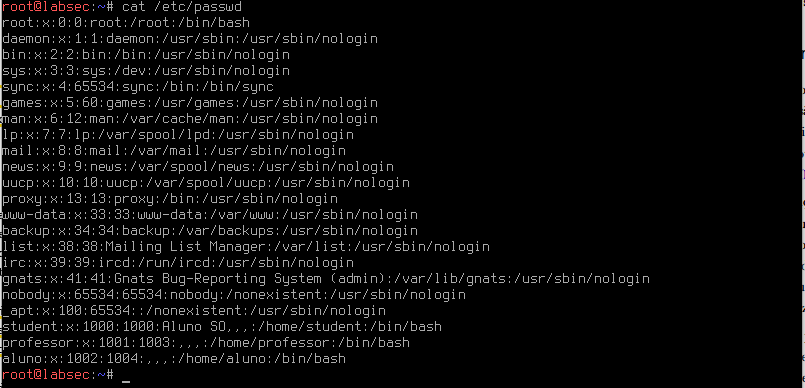
\includegraphics[scale=0.7]{figuras/passwd.png}
  \caption{Arquivo \textit{/etc/passwd}.}
  \label{fig:passwd}
\end{figure}

Para apresentar os campos de dados presentes no arquivo, utilizaremos como exemplo o usuário \textit{student}, os dados presentes no arquivo são:

\begin{itemize}
    \item \textbf{Nome de usuário}: primeiro campo de cada linha, identifica o usuário em questão pelo seu nome de usuário no sistema;
    \item \textbf{Marcador de autenticação}: o segundo campo possui apenas uma marcação ''x`` que significa que a senha do usuário está armazenada no arquivo \textit{/etc/shadow}, caso não haja esta marcação, não será necessário a autenticação para este usuário, a subseção \ref{subsubsec:passwd_root} demonstra melhor o uso deste campo;
    \item \textbf{UID}: o terceiro campo armazena o número de identificação do usuário;
    \item \textbf{GID}: o quarto campo armazena o número de identificação do grupo ao qual o usuário pertence;
    \item \textbf{Informações adicionais}: o quinto campo armazena informações adicionais do usuário, no caso do usuário \textit{student} está armazenado o nome completo do usuário, ''Aluno SO``;
    \item \textbf{Diretório pessoal}: o sexto campo armazena o caminho para o diretório pessoal do usuário, onde ficam seus arquivos no sistema;
    \item \textbf{\textit{shell} padrão}: o sétimo e último campo apresenta o caminho para o executável do \textit{shell} padrão do usuário.
\end{itemize}

\subsection{Gerenciamento de registros}
Um mecanismo presente em sistemas operacionais é a capacidade de realizar registros de atividades realizadas no sistema, chamamos estes registros de registros em \textit{log}. Diversas ações podem ser armazenadas em \textit{logs}, como, por exemplo, cada chamada de sistema realizada, cada usuário autenticado, ou outros comportamentos que podem se tornar suspeitos e serem submetidos a uma futura análise. Estes \textit{logs} são extremamente relevantes, pois auxiliam na detecção de atividades suspeitas que possam indicar uma tentativa de invasão, como falhas de autenticação ou de autorização~\cite{silberschatz2015}.

\subsubsection{Arquivos do diretório \textit{/var/log/}}
O diretório \textit{/var/log/} armazena arquivos de \textit{logs} para prover um melhor controle sobre a segurança do sistema operacional, este diretório armazena diferentes categorias, separadas em diferentes arquivos, como os arquivos:

\begin{itemize}
    \item \textbf{\textit{syslog}}: este arquivo armazena \textit{logs} gerais do sistema, que registra diversos eventos relevantes de categorias que não possuem um arquivo específico para registro;
    \item \textbf{\textit{kern.log}}: este arquivo armazena mensagens originadas no \textit{kernel} do sistema operacional, estas mensagens envolvem eventos como problemas relacionados ao hardware ou até mesmo de mau funcionamento do núcleo;
    \item \textbf{\textit{auth.log}}: este arquivo armazena \textit{logs} relacionados à autenticação de usuários, como tentativas de \textit{login} ou mudança de privilégios por meio do comando \textit{sudo};
    \item \textbf{\textit{daemon.log}}: este arquivo armazena mensagens provenientes de \textit{daemons}, que são processos do sistema sendo executados em segundo plano, o que se torna relevante devido à execução discreta destes processos, que não interagem com o usuário.
\end{itemize}

\subsubsection{Configuração do arquivo \textit{/etc/logrotate.conf}}
Sistemas operacionais Linux possuem uma ferramenta chamada \textit{logrotate}, que automatiza algumas atividades referentes aos \textit{logs}, como a rotação e gerenciamento de histórico de \textit{logs}. Esta ferramenta pode ser configurada alterando o arquivo \textit{/etc/logrotate.conf} conforme a necessidade, a atividade propõe a duas configurações importantes, a rotação diária de \textit{logs}, e o armazenamento de três meses de histórico. Na prática, isso implica na criação de um novo arquivo de \textit{log} todo dia, e o armazenamento dos últimos 90 arquivos (3 meses).

Para aplicar a configuração proposta, o arquivo \textit{/etc/logrotate.conf} foi alterado, utilizando o editor de texto \textit{Nano}, e a rotação foi alterada para ''\textit{daily}`` (diária) e o armazenamento foi alterado para ''\textit{rotate} 90``, para armazenar 90 rotações. Este arquivo alterado pode ser observado na figura \ref{fig:logrotate}.

\begin{figure}[H]
  \centering
  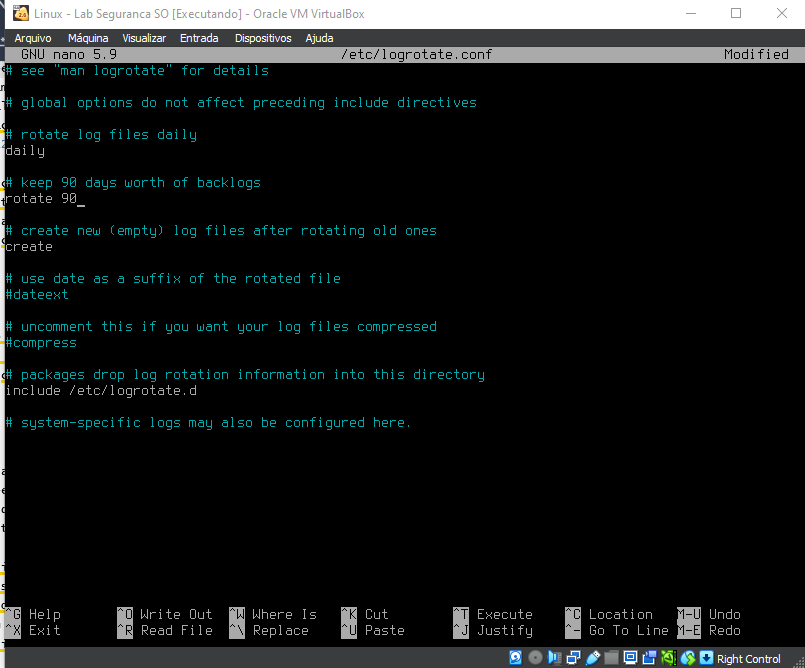
\includegraphics[scale=0.7]{figuras/logrotate.png}
  \caption{Arquivo \textit{/etc/logrotate.conf}.}
  \label{fig:logrotate}
\end{figure}

\subsubsection{Identificação de serviços ativos}

Outra atividade importante no âmbito na segurança em sistemas operacionais é a observação dos serviços ativos no sistema, pois permite a identificação de serviços suspeitos, que poderiam acarretar falhas de segurança como roubo de serviço ou recusa de serviço, citadas na seção \ref{sec:fundamentacao}.

A verificação dos serviços de um sistema operacional Linux pode ser realizada com o auxílio do comando \textit{service}, acompanhado da opção ''\textit{--status-all}``, e para filtrar os serviços ativos podemos redirecionar a saída do comando anterior para o comando \textit{grep}, responsável por filtrar as linhas que contenham um determinado texto, como todo serviço ativo possui o marcador ''[ + ]`` em sua linha, vamos utilizar este termo para filtrar, o resultado desta operação pode ser visualizado na figura \ref{fig:service}.

\begin{figure}[H]
  \centering
  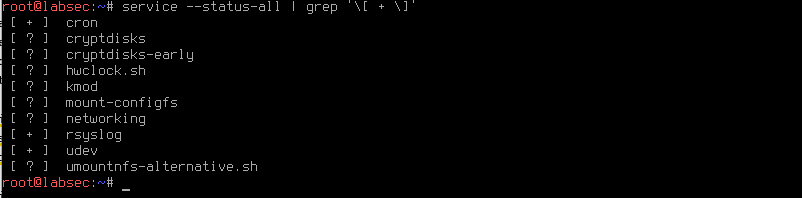
\includegraphics[scale=0.7]{figuras/service.png}
  \caption{Comando \textit{service}.}
  \label{fig:service}
\end{figure}

Devido à forma que o \textit{grep} interpreta caracteres especiais, os serviços com status indefinidos, demarcados com ''[ ? ]`` também são retornados, mas pode-se ignorá-los.

\subsection{Outros mecanismos de segurança}
O problema da segurança em sistemas operacionais é amplamente discutido e a comunidade busca constantemente soluções nesta área, algumas soluções importantes que visam serão apresentadas a seguir.

\subsubsection{SELinux}
O SELinux é um mecanismo de controle de acesso multipolíticas, que constitui uma infraestrutura de segurança para o núcleo Linux, permitindo a aplicação de políticas diversas aos recursos do sistema operacional. Uma desvantagem desta infraestrutura é sua alta complexidade, que torna sua compreensão e configuração difícil, devido a este fator, outros sistemas que visam o mesmo objetivo vem sendo desenvolvidos buscando uma complexidade menor para se tornarem mais simples de se aplicar ao núcleo Linux~\cite{maziero2019}.

\subsubsection{\textit{Pluggable Authentication Modules}}
Outro recurso disponível no Linux é o PAM (\textit{Pluggable Authentication Modules}) é um mecanismo baseado em uma biblioteca compartilhada que pode ser utilizada por qualquer componente do sistema operacional que precise realizar a autenticação de usuários para a realização de alguma atividade. O funcionamento do PAM permite o carregamento de módulos de autenticação conforme especificado no arquivo de configurações, esta modularização permite que novos módulos sejam adicionados na configuração e em seguida já esteva, disponíveis para qualquer componente do sistema~\cite{silberschatz2015}.

\section{Discussão dos Resultados}
\label{sec:discussao}

Os resultados obtidos foram satisfatórios, alcançando o objetivo de compreender e aplicar conceitos e recursos de segurança em sistemas operacionais Linux com sucesso. O processo não proporcionou grandes dificuldades, apenas uma curva de aprendizado um pouco acima do esperado, que foi superada com o auxílio da bibliografia. Foi possível realizar com êxito configurações importantes relacionadas a segurança, como a implementação de requisitos para as senhas, atribuição de permissões a arquivos e remoção de usuários do grupo \textit{sudo}. Além disso, foi possível identificar e conhecer arquivos importantes para a segurança do sistema operacional.

\section{Conclusões}
\label{sec:conclusoes}

O objeto do trabalho de compreender e aplicar conceitos e recursos de segurança em sistemas operacionais foi atingido com sucesso e sua importância para a segurança da informação ficou clara ao longo do processo. Durante os procedimentos foram realizadas configuração e verificação de arquivos importantes para a segurança em sistemas operacionais Linux. O aprendizado obtido durante o trabalho é de fundamental importância para a formação de um cientista da computação, visto que sistemas operacionais são amplamente utilizados e podem se tornar alvos de invasores, comprometendo a segurança da informação. Além de todos os procedimentos realizados, ainda há diversos recursos de segurança não explorados durante a atividade e que podem prover meios eficazes de proteger dados e recursos.

% ----------------------------------------------------------
% ELEMENTOS PÓS-TEXTUAIS
% ----------------------------------------------------------
\postextual
% ----------------------------------------------------------
% Referências bibliográficas
% ----------------------------------------------------------
\renewcommand{\bibsection}{%
\section{\bibname}
\bibmark
%\ifnobibintoc\else
%\phantomsection
%\addcontentsline{toc}{section}{\bibname}
%\fi
\prebibhook}

\bibliography{abntex2-modelo-references}

\end{document}
